
\section{Adversarial Attack}
\label{attack}
In this section, we will first introduce the definition of adversarial attack against deep learning methods on graphs. Then,  we categorize these attack models from different perspectives. Finally, we will give a clear overview on existing works.

\subsection{Definition}
\label{attackDefinition}
According to existing works on graph adversarial attacks, we summarize and give a unified formulation for them.

\nosection{Attack on Graph Data} Considering $f$ a deep learning function designed to tackle related downstream tasks. Given a set of target instances $\mathcal{T} \subseteq \mathcal{S}-\mathcal{S}_L$, where $\mathcal{S}$ could be $\mathcal{V}$, $\mathcal{E}$ or $\mathcal{G}$ respectively for different levels of tasks, and $\mathcal{S}_L$ denotes the instances with labels,\footnote{Note that attackers only focus on attacking the target instances in the test set.} the attacker aims to maximize the loss of the target node on $f$ as much as possible, resulting in the degradation of prediction performance. Generally, we can define the attack against deep learning models on graphs as:

\begin{equation}
	\label{definition}
	\begin{split}
		& \underset{\hat{G} \in \Psi(G)}{\text{maximize}} \sum_{t_i \in \mathcal{T}} \mathcal{L}(f_{\theta^{\ast}}(\hat{G}^{t_i}, X, t_i), y_i)  \\
		& s.t. \ \theta^{\ast} = \mathop{\arg \min}_{\theta} \sum_{v_j \in \mathcal{S}_L}\mathcal{L}(f_{\theta}(\tilde{G}^{v_j}, X, t_j)), y_j)
	\end{split}
\end{equation}

We denote a graph $G \in \mathcal{G}$ with node $t_i$ in it as $G^{t_i}$. $\hat{G}$ denotes the perturbed graph and $\Psi(G)$ indicates the perturbation space on $G$, and we use $\tilde{G}$ to represent original graph $G$ or a modified one $\hat{G}$, respectively.

To make the attack as imperceptible as possible, we set a metric for comparison between the graphs before and after the attack, such that:
\begin{equation}
	\begin{split}
		\mathcal{Q}(\hat{G}^{t_i}, G^{t_i}) < \epsilon \\ s.t.\ \hat{G}^{t_i} \in \Psi(G)
	\end{split}
\end{equation}
where $\mathcal{Q}$ denotes a similarity function, and $\epsilon$ is an allowed threshold of changes. Specifically, more metrics will be detailed in Section \ref{metrics}.


\subsection{Taxonomies of Attacks}
As we focus on a simple graph, different types of attacks could be conducted on the target systems. In this section, we provide taxonomies for the attack types mainly proposed by Sun et al. \cite{sun2018adversarial} and subsequently extended in our works according to various criteria. For different scenarios, we give relevant instructions and summarize them in the following:

\subsubsection{Attacker’s Knowledge}
To conduct attacks on the target system, usually an attacker will possess certain knowledge about the target models and the dataset, which helps them achieve the adversarial goal. Based on the knowledge of the target models \cite{sun2018adversarial}, we characterize different threatening levels of attacks.
\nosection{\textbf{White-box Attack}}
This is the simplest attacks while attackers possess the entire information of the target models, including the model architecture, parameters and gradient information, i.e., the target models are fully exposed to the attackers. By utilizing such rich information, attackers can easily affect the target models and bring destructive effects. However, it is impracticable in real world since it is costly to possess such complete knowledge of target models. Therefore white-box attack is less dangerous but often used to approximate the worst performance of a system under attack.
\nosection{\textbf{Gray-box Attack}}
In this case, attackers are strict to possess excessive knowledge about the target models, this reflects real world scenarios much better since it is more likely that attackers have limited access to get the information, e.g., only familiar with the architecture of the target models. Therefore, it's harder than conducting the white-box attack but more dangerous for the target models.
\nosection{\textbf{Black-box Attack}}
In contrast to white-box attack, black-box attack assumes that the attacker does not know anything about the targeted systems. Under this setting, attackers are only allowed to do black-box queries on limited samples at most. However, it will be the most dangerous attack once it works, since attackers can attack any models with limited (or no) information.

Here also comes a term \textbf{``no-box attack''} \cite{sharma2018gradient} which refers to an attack on the surrogate model based on their (limited) understanding of the target model.\footnote{We must realize that no-box is a kind of gray- or black-box attack so we don't don't have a separate category for it.} As attackers have complete knowledge of the surrogate model, the adversarial examples are generated under white-box setting. No-box attack will become a white-box attack once the attackers build a surrogate model successfully and the adversarial examples are transferable to fool other target models. Theoretically, this kind of attack can hardly affect the systems in most cases with these constraints. However, as if the surrogate model has strong transferability, the no-box attack is also destructive.

As attackers are strict with the knowledge of the target models, they also have less access to the information of the dataset $\mathcal{D}$. Based on the different levels of knowledge of the targeted system \cite{chen2017practical}, we have:
\nosection{\textbf{Perfect Knowledge}}
In this case, the dataset $\mathcal{D}$, including the entire graph structure, node features, and even the ground-truth labels of objects, are completely exposed to attackers, i.e., the attacker is assumed to know \emph{everything} about the dataset. This is impractical but the most common setting in previous studies. However, considering the damage that could be done by an attacker with perfect knowledge is critical, since it may expose the potential weaknesses of the target system in a graph.

\nosection{\textbf{Moderate Knowledge}}
The moderate knowledge case represents an attacker with less information about the dataset. This makes attackers focus more on the performance of their attacks, or even search for more information through legitimate or illegitimate methods.

\nosection{\textbf{Minimal Knowledge}}
This is the hardest one as attackers can only conduct attacks with the minimal knowledge of datasets, such as partial connections of the graph or the feature information of certain nodes. This is essential information for an attacker, otherwise it will fail even under the white-box attack setting. The minimal knowledge case represents the least sophisticated attacker and naturally with less threat level.

To conclude, we use $\mathcal{K}$ to denote the attackers' knowledge in an abstract knowledge space. Here $\mathcal{K}$ is consisting of three main parts, the dataset knowledge, the training algorithm and the learned parameters of target models. For instance, $\mathcal{K}=(\mathcal{D},f,\theta)$ denotes white-box attack with perfect knowledge, and $\mathcal{K}=(\mathcal{D}_{train},\hat{f},\hat{\theta})$ denotes gray- or black-box attack and with moderate knowledge, where $\hat{f}$ and $\hat{\theta}$ come from the surrogate model and $\mathcal{D}_{train}\subset \mathcal{D}$ denotes the training dataset.

\begin{figure}
	\centering
	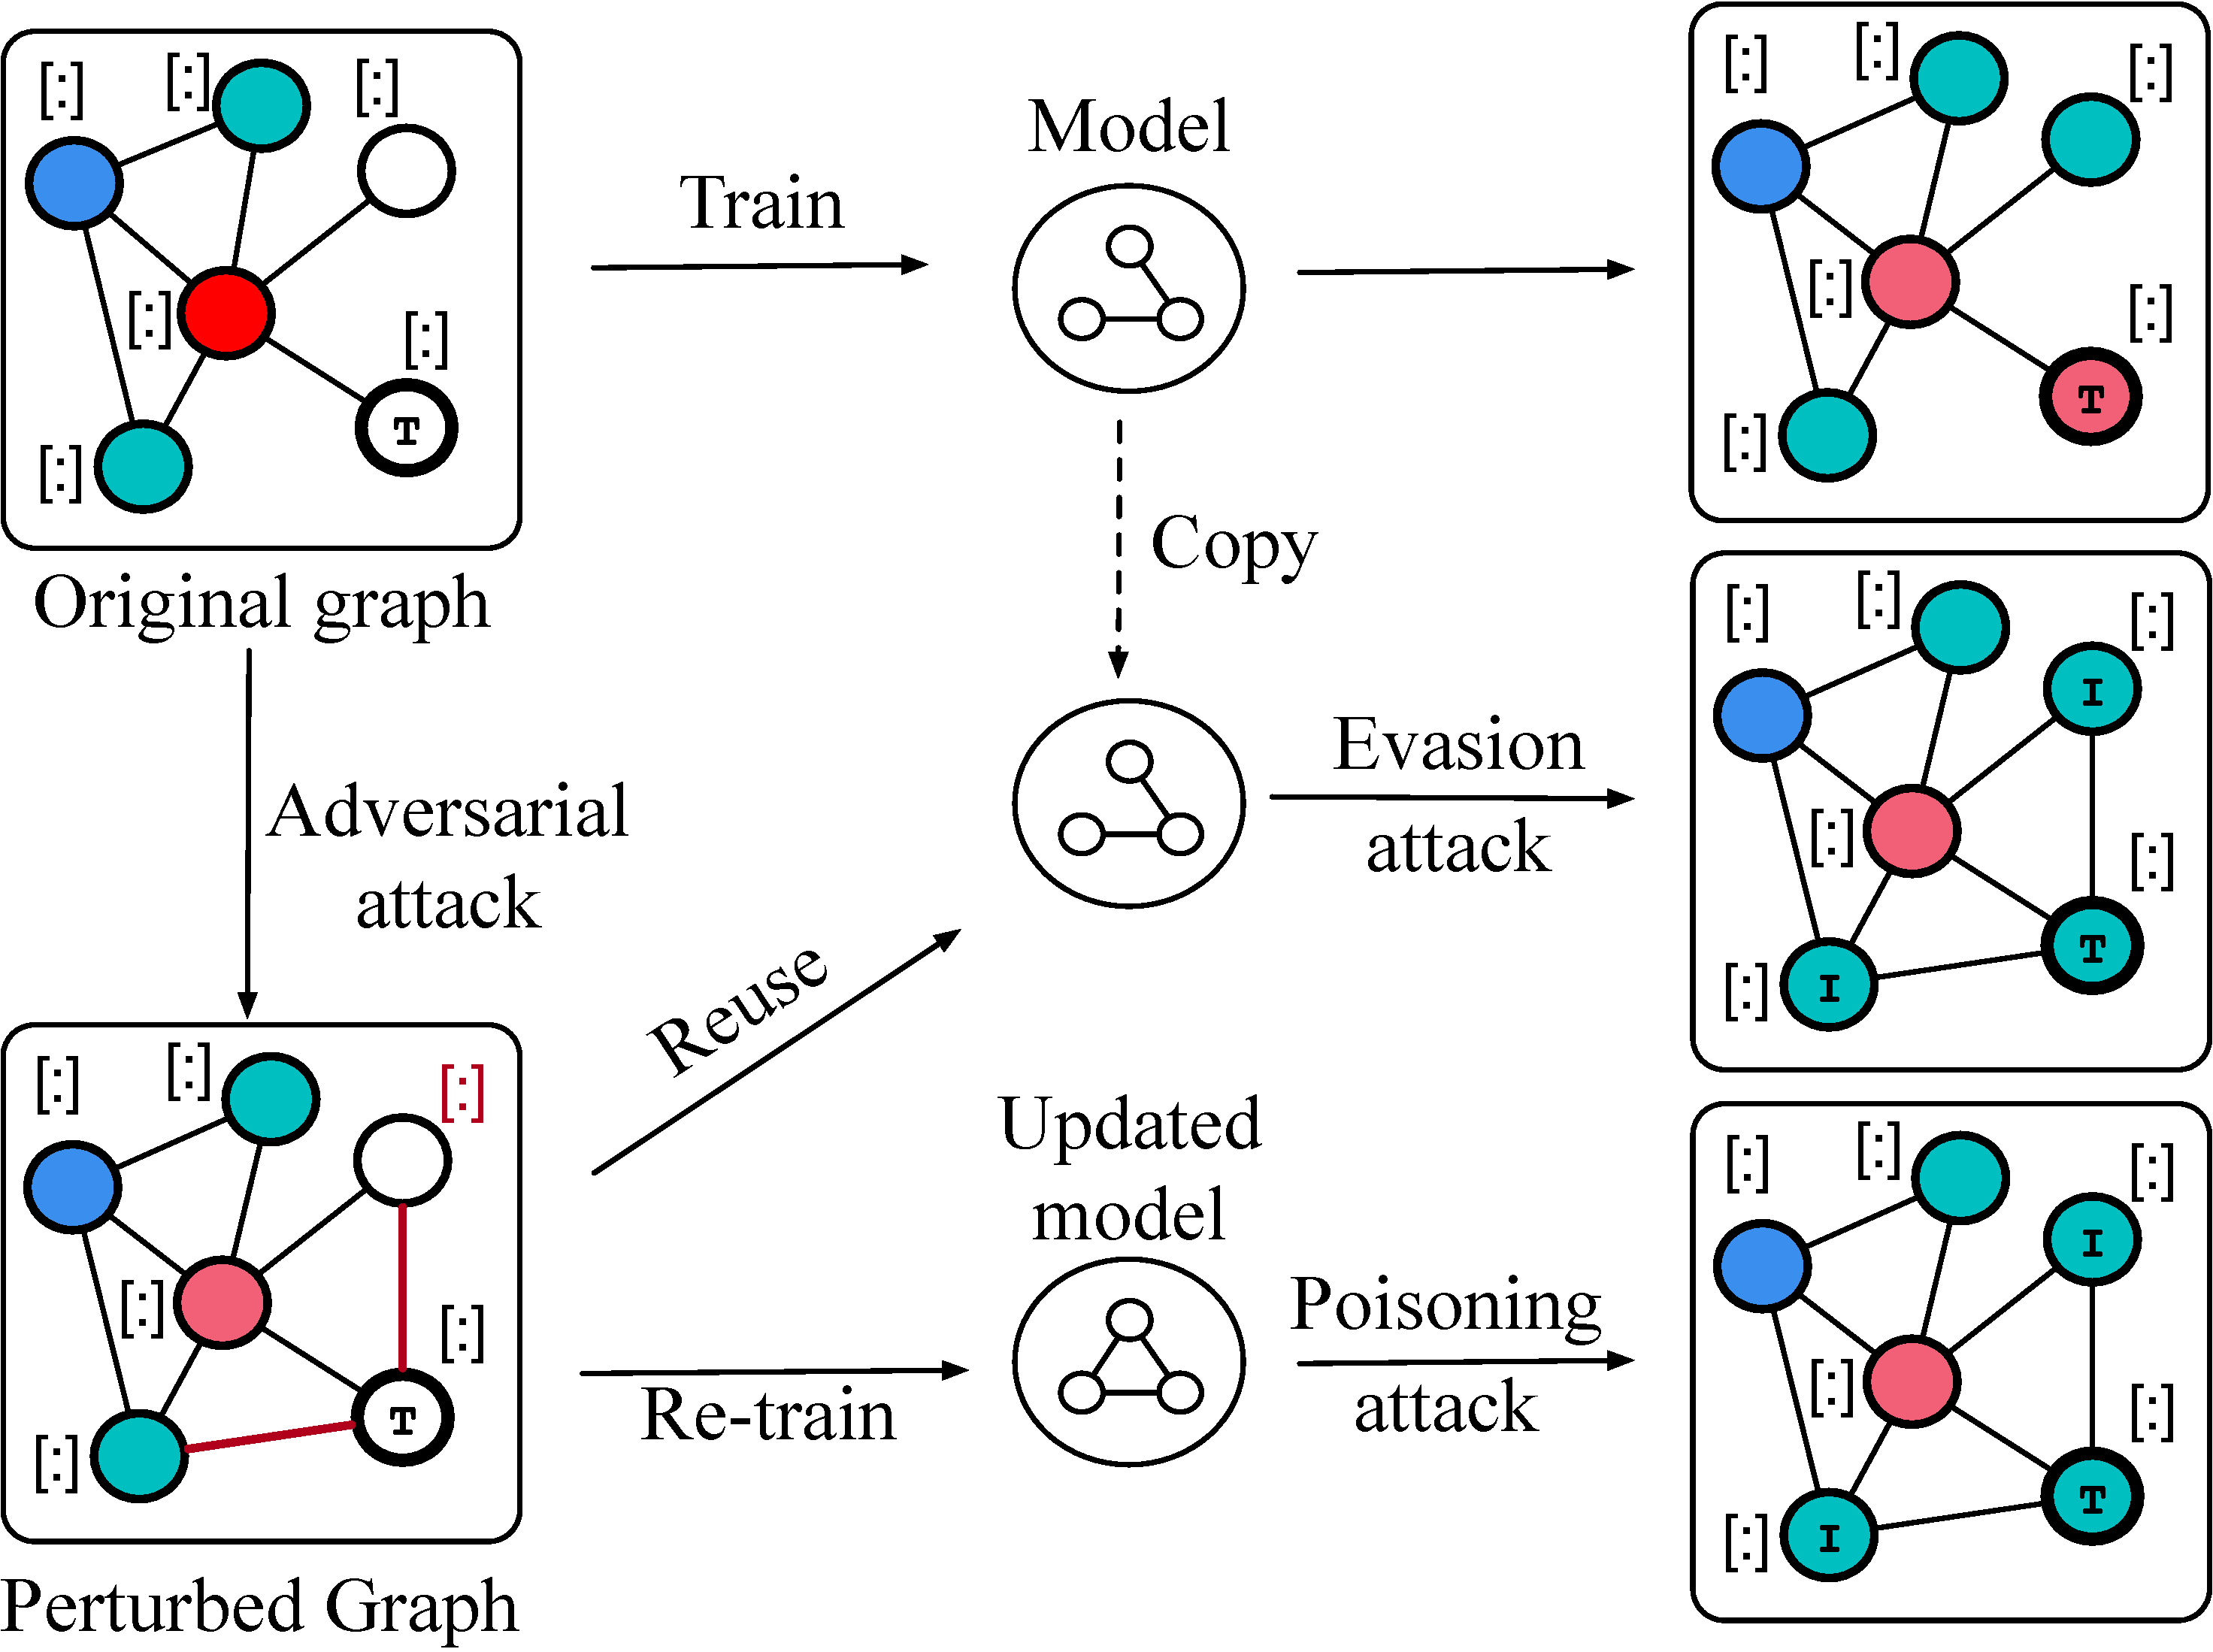
\includegraphics[width=70mm]{EvasionPoisoning.pdf}
	\caption{An example of the evasion attack and the poisoning attack. (Image Credit: Z{\"u}nger et al. \protect\cite{zugner2018adversarial}) }
	\label{Fig2}
\end{figure}

\subsubsection{Attacker's Goal}
The goal generally distinguishes three different types of attacks, i.e., \emph{security violation}, \emph{attack specificity} and \emph{error specificity} \cite{biggio2018wild}.	They are not mutually exclusive in fact, and more details are discussed below.

\nosection{\textbf{Security Violation}}
Security violation can be categorized into \emph{availability attack}, \emph{integrity attack} and \emph{others}. For availability attack, the the attacker attempts to destroy the function of the system, thereby impairing its normal operation. The damage is global, that is, it attacks the overall performance of the whole system. For integrity attack, the attackers' purpose is to bypass or fool the detection of the system, which is different from availability attack in that it does not destroy the normal operation of the system. There are other goals, such as reverse-engineering model information to gain privacy knowledge.

\nosection{\textbf{Error Specificity}}
Take node classification task as an example, the error specific attack aims to misclassify the predictions as specific labels, while unspecific attack does not care what the prediction is, the attack is considered successful as long as the prediction is wrong.

\nosection{\textbf{Attack Specificity}}
This perspective focuses on the range of the attack, which can divide attacks into \emph{targeted attack} and \emph{non-targeted attack (general attack)}. The targeted attack focuses on a specific subset of nodes (usually a target node), while the non-targeted attack is undifferentiated and global. With reference to Eq.(\ref{definition}), the difference is the domain of $\mathcal{T} \subset \mathcal{S} - \mathcal{S}_L$ or $\mathcal{T} = \mathcal{S} - \mathcal{S}_L$.

It is worth noting that in some other fields (e.g., computer vision), \emph{targeted attack} refers to the specific error attack, and \emph{non-targeted attack} the unspecific error attack. In the field of graph adversarial learning, we suggest that distinguishing the targeted attack based on the attack range, and whether it is error specific based on the consequence.

\subsubsection{Attacker's Capability}
\label{period}
Attacks can be divided into poisoning attack and evasion attack according to adversaries' capabilities, which are occurred at different stages of the attacks.
\nosection{\textbf{Poisoning Attack}}
Poisoning attacks (a.k.a training-time attacks) try to affect the performance of the target models by modifying the dataset in the training stage, i.e., the target models are trained on the poisoned datasets. Since transductive learning is widely used in most graph analysis tasks, the test samples (but not their labels) are participated in the training stage, which leads to the popularity of poisoning attacks. Under this scenario, the parameters of target models are retrained after the training dataset being modified, thus we can define poisoning attacks according to Eq.(\ref{definition}):
\begin{equation}
	\label{poisoning}
	\begin{aligned}
		 & \underset{\hat{G} \in \Psi(G)} {\text{maximize}} \sum_{t_i \in \mathcal{T}} \mathcal{L}(f_{\theta^*}(\hat{G}^{t_i},X,t_i),y_i)   \\
		 & s.t. \ \theta^{\ast} = \mathop{\arg \min}_{\theta} \sum_{v_j \in \mathcal{S}_L}\mathcal{L}(f_{\theta}(\hat{G}^{v_j},X,v_j), y_j)
	\end{aligned}
\end{equation}

\nosection{\textbf{Evasion Attack}}
While poisoning attacks focus on the training phase, evasion attacks (a.k.a test-time attacks) tend to add adversarial examples in test time. Evasion attacks occur after the target model is well trained on a clean graph, i.e., the learned parameters are fixed during evasion attacks. Therefore, we can define the formulation of evasion attacks by changing part of Eq.(\ref{poisoning}) slightly:
\begin{equation}
	\begin{aligned}
		\theta^{\ast} = \mathop{\arg \min}_{\theta} \sum_{v_j \in \mathcal{S}_L}\mathcal{L}(f_{\theta}(G^{v_j},X,v_j), y_j)
	\end{aligned}
\end{equation}

In Figure \ref{Fig2}, we show a toy example of the poisoning attack and the evasion attack. In most cases the poisoning attack does not work well because the model is retrained to alleviate the adversarial impacts.

\subsubsection{Attack Strategy}
For attacking a target model on graph data, attackers may have a line of strategies to achieve their adversarial goals. In most instances, they will focus on the graph structure or node/edge features. Based on the strategy applied on a graph, we have:
\nosection{\textbf{Topology Attack}}
Attackers are mainly focus on the the topology of the graph, a.k.a, structure attack. For example, they are allowed to add or remove some edges legally between nodes in the graph to fool the target system. To specify this, we define an attack budget $\Delta \in \mathbb{N}$, thus the definition of the topology attack is:
\begin{equation}
	\begin{aligned}
		 & \underset{\hat{G} \in \Psi(G)} {\text{maximize}} \sum_{t_i \in \mathcal{T}} \mathcal{L}(f_{\theta^*}(\hat{G}^{t_i},X,t_i),y_i) \\
		 & s.t. \  \sum_{u<v} |A_{u,v}-A'_{u,v} | \leq \Delta
	\end{aligned}
\end{equation}
where $A'$ is the adjacency matrix of the perturbed graph, and $\theta^*$ is discussed in Section \ref{period}.

\nosection{\textbf{Feature Attack}}
Although the topology attack is more common, attackers can conduct feature attacks as well. Under this setting, the features of specified objects will be changed. However, unlike graph structure, the node/edge features could be either binary or continuous, i.e., $X \in \{0,1\}^{N \times F_{(\cdot)}}$ or $X \in \mathbb{R}^{N \times F_{(\cdot)}}$. For binary features, attackers can flip them like edges, while for continuous features, attackers can add a small value on them, respectively. Thus the definition of feature attacks is:
\begin{equation}
	\begin{aligned}
		 & \underset{\hat{G} \in \Psi(G)} {\text{maximize}} \sum_{t_i \in \mathcal{T}} \mathcal{L}(f_{\theta^*}(\hat{G}^{t_i},X,t_i),y_i) \\
		 & s.t. \  \sum_u \sum_j  |X_{u,j}-X'_{u,j} | \leq \Delta
	\end{aligned}
\end{equation}
where $X'$ is similarly defined, and  here $\Delta \in \mathbb{N}$ for binary features and $\Delta \in \mathbb{R}$ for continuous features.

\nosection{\textbf{Hybrid}}
Usually, attackers will conduct both attack strategies at the same time to exert more powerful impact. Besides, they could even add several fake nodes (with fake labels), which will have their own features and relationship with other benign instances. For example, some fake users will be added into the recommendation system and affect the results of the system \cite{chen2019data,hou2019alphacyber}. Therefore, we conclude a unified formulation as follows:
\begin{equation}
	\begin{aligned}
		 & \underset{\hat{G} \in \Psi(G)} {\text{maximize}} \sum_{t_i \in \mathcal{T}} \mathcal{L}(f_{\theta^*}(\hat{G}^{t_i},X,t_i),y_i) \\
		 & s.t. \  \sum_{u<v} |A_{u,v}-A'_{u,v} | + \sum_u \sum_j  |X_{u,j}-X'_{u,j} |\leq \Delta
	\end{aligned}
\end{equation}
$A'$ and $X'$ may not have the same dimension with $A$ and $X$ respectively if some fake nodes are added into the graph.

\subsubsection{Attacker’s Manipulation}
Although attackers may have enough knowledge about the target system, they may not always have access to manipulation all of the dataset. Besides, different manipulations may have different budget cost. For example, in an e-commerce system \cite{DBLP:conf/ijcai/ChenL0GZ19}, attackers could only purchase more items (add edges) but unable to delete the purchase records (remove edges). Based on different manipulation, we have:
\nosection{\textbf{Add}}
In a graph, attackers could add edges between different nodes, or add features on specified nodes/edges. This is the most simplest manipulation and naturally has lowest budget in most scenarios.
\nosection{\textbf{Remove}}
In a graph, attackers could remove edges between different nodes, or remove features on specified nodes/edges. This kind of manipulation will be harder than ``add'', since attackers may not have enough access to execute the ``remove'' manipulation.
\nosection{\textbf{Rewiring}}
The manipulations mentioned above may become more noticeable for the target system if $\Delta$ is larger. To address this problem, the rewiring operation is proposed in a less noticeable way than simple adding/removing manipulation \cite{ma2019attacking, waniek2018attack}. For instance, attackers can add an edge connected with a target node, while remove an edge connected with it at the same time. Each time of rewiring manipulation related to two single operations, which can preserve some basic graph properties (e.g., degree) and naturally more unnoticeable.

To conclude, we define an operation set $\mathcal{O}=\{\mathcal{O}_{Add},\mathcal{O}_{Rem},\mathcal{O}_{Rew}\}$, representing the above three manipulations of attackers, respectively.

\subsubsection{Attack Algorithm}
Generally speaking, current methods of adversarial attacks on generating adversarial examples are mainly based on the gradient information, either from the target model (white-box attack) or the surrogate model (black- or gray-box attack). Beyond that, there are several methods generating adversarial examples based on other algorithms. From the perspective of attack algorithm, we have:
\nosection{\textbf{Gradient-based Algorithm}}
Intuitively, gradient-based algorithm is simple but effective. The core idea is that: fix the parameters of a trained model, and regard the input as a hyperparameter to optimize. Similar to the training process, attackers could use the partial derivative of loss $\mathcal{L}$ with respect to edges (topology attack) or features (feature attack), to decide how to manipulate the dataset. However, gradients could not applied directly into the input data due to the discreteness of the graph data, instead, attackers often choose the one with greatest absolute gradients, and manipulate it with a proper value. While most deep learning models are optimized by gradients, on the contrary, attackers could destroy them by gradients as well.

\nosection{\textbf{Non-gradient-based Algorithm}}
In addition to gradient information, attackers could generate adversarial examples in other ways. For example, from the perspective of the genetic algorithm, attackers can choose the population (adversarial examples) with highest fitness score (e.g., erroneous outputs of the target/surrogate model) generations by generations. Besides, reinforcement learning algorithms are also commonly used to solve this issue. Reinforcement learning based attack methods \cite{dai2018adversarial,ma2019attacking} will learn the generalizable adversarial examples within an action space. Moreover, adversarial examples can even generated by a well-designed generative model.

\subsubsection{Target Task}
As discussed in Section \ref{task}, there exists three major tasks in graph domains. According to different levels of tasks, we can divide existing attack methods into the following three categories, respectively.

\nosection{\textbf{Node-relevant Task}}
Currently, there are several attack models against node-relevant tasks \cite{zugner2018adversarial,bojchevski2019adversarial,xu2019topology,zugner2019adversarial,wang2018attack,chen2018fast,dai2018adversarial,dai2018adversarial,xuan2019unsupervised,bose2019generalizable,wang2019attacking,waniek2018attack,chen2018link,sun2018data,zhou2019attacking,wu2019adversarial}. Typically, Bojchevski et al. and Hou et al. \cite{bojchevski2019adversarial,hou2019alphacyber} utilize random walk \cite{perozzi2014deepwalk} as an surrogate model to attack node embedding,  Dai et al. \cite{dai2018adversarial} uses a reinforcement learning based framework to disturb node classification tasks. In general, most of the existing works address in node classification task due to its ubiquity in real world.
%Most of the existing methods are still transductive, since the nodes on the graph are not independent with their neighbors. 
%For example, common Graph Neural Network (GNN) related algorithms take the information around the nodes into full consideration. 

\nosection{\textbf{Link-relevant Task}}
Many relationships in real world can be represented by graph. For some of these graphs, such as social graph, are always dynamic in reality. Therefore, the link prediction on the graph comes into being, in order to predict the change of the edge. Link prediction is also the most common application of link-relevant tasks and there are many attack related studies have been proposed \cite{chen2018link,waniek2018attack,zhou2019attacking,sun2018data,zhou2019attacking,chen2019data,christakopoulou2018adversarial,chen2019time}.

\nosection{\textbf{Graph-relevant Task}}
Graph-relevant tasks treat graph as a basic unit. Compared to node- or link-relevant tasks, it is macro and large-scale. The application of graph-relevant methods are more inclined to the research community of biology, chemistry, environment, materials, etc. In this task, the model tries to extract features of nodes and spatial structures to represent a graph, so as to achieve downstream operations such as graph classification or clustering. Similar with  Eq.(\ref{definition}), the targets of attack should be an graphs, while $y$ is determined by the specific task. For graph-relevant tasks, some attack researches have also appeared \cite{ma2019attacking,chen2019ga,chen2017practical}.

\begin{table*}[]
	\centering
	\caption{Related works on attack in details.}
	\label{attack_table}
	\scalebox{0.75}{
		\begin{tabular}{c|cccccccccc}
			\hline
			\hline
			Reference                             &
			Model                                 &
			Algorithm                             &
			Target Task                           &
			Target Model                          &
			Baseline                              &
			Metric                                &
			Dataset                               & \\

			\hline
			\cite{chang2019restricted}            &
			\begin{tabular}[c]{@{}c@{}} GF-Attack \end{tabular}            &
			\begin{tabular}[c]{@{}c@{}} Graph signal processing\end{tabular}            &
			\begin{tabular}[c]{@{}c@{}} Node classification \end{tabular}            &
			\begin{tabular}[c]{@{}c@{}} GCN, SGC,\\DeepWalk, LINE \end{tabular}            &
			\begin{tabular}[c]{@{}c@{}} Random, \\Degree, \\RL-S2V,\\ $A_{class}$ \end{tabular}            &
			\begin{tabular}[c]{@{}c@{}} Accuracy \end{tabular}            &
			\begin{tabular}[c]{@{}c@{}} Cora,\\Citeseer,\\Pubmed \end{tabular}              \\

			\hline
			\cite{wu2019adversarial}              &
			\begin{tabular}[c]{@{}c@{}} IG-FGSM,\\IG-JSMA \end{tabular}            &
			\begin{tabular}[c]{@{}c@{}} Gradient-based GCN\end{tabular}            &
			\begin{tabular}[c]{@{}c@{}} Node classification \end{tabular}            &
			\begin{tabular}[c]{@{}c@{}} GCN \end{tabular}            &
			\begin{tabular}[c]{@{}c@{}} FGSM,\\ JSMA,\\ Nettack \end{tabular}            &
			\begin{tabular}[c]{@{}c@{}} Classification margin,\\Accuracy \end{tabular}            &
			\begin{tabular}[c]{@{}c@{}} Cora,\\Citeseer,\\PolBlogs \end{tabular}              \\

			\hline
			\cite{chen2019multiscale}             &
			\begin{tabular}[c]{@{}c@{}} EPA \end{tabular}            &
			\begin{tabular}[c]{@{}c@{}} Genetic algorithm \end{tabular}            &
			\begin{tabular}[c]{@{}c@{}} Community detection \end{tabular}            &
			\begin{tabular}[c]{@{}c@{}} GRE, INF,\\ LOU \end{tabular}            &
			\begin{tabular}[c]{@{}c@{}} $A_Q$, $A_S$, $A_B$,\\$A_D$, $D_S$, $D_W$ \end{tabular}            &
			\begin{tabular}[c]{@{}c@{}} NMI,\\ ARI \end{tabular}            &
			\begin{tabular}[c]{@{}c@{}} Synthetic networks,\\Football, Email, \\Polblogs \end{tabular}              \\

			\hline
			\cite{zugner2019adversarial}          &
			\begin{tabular}[c]{@{}c@{}} Meta-Self, \\Meta-Train \end{tabular}            &
			\begin{tabular}[c]{@{}c@{}} Gradient-Based GCN \end{tabular}            &
			\begin{tabular}[c]{@{}c@{}} Node  classification \end{tabular}            &
			\begin{tabular}[c]{@{}c@{}} GCN,\\CLN,\\Deepwalk \end{tabular}            &
			\begin{tabular}[c]{@{}c@{}} DICE,\\Nettack,\\First-order \end{tabular}           &
			\begin{tabular}[c]{@{}c@{}} Misclassification rate,\\Accuracy \end{tabular}           &
			\begin{tabular}[c]{@{}c@{}} Cora-ML,\\Citeseer,\\PolBlogs,\\PubMed, \end{tabular}             \\

			\hline
			\cite{bojchevski2019adversarial}      &
			\begin{tabular}[c]{@{}c@{}} $\mathcal{A}_{DW2}$,\\$\mathcal{A}_{DW3}$ \end{tabular}           &
			\begin{tabular}[c]{@{}c@{}} Gradient-based random walk \end{tabular}           &
			\begin{tabular}[c]{@{}c@{}}Node classification,\\Link prediction\end{tabular}           &
			\begin{tabular}[c]{@{}c@{}} Deepwalk \end{tabular}           &
			\begin{tabular}[c]{@{}c@{}}$\mathcal{B}_{rnd}$\\$\mathcal{B}_{eig}$\\$\mathcal{B}_{deg}$ \end{tabular}           &
			\begin{tabular}[c]{@{}c@{}} F1 score,\\Classification margin \end{tabular}           &
			\begin{tabular}[c]{@{}c@{}}Cora,\\Citeseer,\\PolBlogs\end{tabular}             \\

			\hline
			\cite{chen2019time}                   &
			\begin{tabular}[c]{@{}c@{}} TGA-Tra,\\ TGA-Gre \end{tabular}           &
			\begin{tabular}[c]{@{}c@{}} Gradient-based DDNE \end{tabular}           &
			\begin{tabular}[c]{@{}c@{}}Link prediction\end{tabular}           &
			\begin{tabular}[c]{@{}c@{}} DDNE,\\ctRBM,\\GTRBM,\\dynAERNN \end{tabular}           &
			\begin{tabular}[c]{@{}c@{}}Random, \\DGA,\\CNA \end{tabular}           &
			\begin{tabular}[c]{@{}c@{}} ASR, AML \end{tabular}           &
			\begin{tabular}[c]{@{}c@{}}RADOSLAW,\\LKML,\\FB-WOSN\end{tabular}             \\

			\hline
			\cite{ma2019attacking}                &
			\begin{tabular}[c]{@{}c@{}} ReWatt \end{tabular}           &
			\begin{tabular}[c]{@{}c@{}} Reinforcement learning\\based on GCN \end{tabular}           &
			\begin{tabular}[c]{@{}c@{}} Graph\\classification \end{tabular}           &
			\begin{tabular}[c]{@{}c@{}} GCN \end{tabular}           &
			\begin{tabular}[c]{@{}c@{}} RL-S2V,\\Random \end{tabular}           &
			\begin{tabular}[c]{@{}c@{}} ASR \end{tabular}           &
			\begin{tabular}[c]{@{}c@{}} REDDIT-\\MULTI-12K,\\REDDIT-MULTI-5K,\\IMDB-MULTI \end{tabular}             \\

			\hline
			\cite{xu2019topology}                 &
			\begin{tabular}[c]{@{}c@{}} PGD,\\Min-Max \end{tabular}           &
			\begin{tabular}[c]{@{}c@{}} Gradient-based GCN \end{tabular}           &
			\begin{tabular}[c]{@{}c@{}} Node classification \end{tabular}           &
			\begin{tabular}[c]{@{}c@{}} GCN \end{tabular}           &
			\begin{tabular}[c]{@{}c@{}} DICE,\\Meta-Self,\\Greedy \end{tabular}           &
			\begin{tabular}[c]{@{}c@{}} Misclassification\\rate \end{tabular}           &
			\begin{tabular}[c]{@{}c@{}} Cora,\\Citeseer \end{tabular}             \\

			\hline
			\cite{xuan2019unsupervised}           &
			\begin{tabular}[c]{@{}c@{}} EDA \end{tabular}           &
			\begin{tabular}[c]{@{}c@{}} Genetic algorithm\\based on Deepwalk \end{tabular}           &
			\begin{tabular}[c]{@{}c@{}} Node classification,\\Community detection \end{tabular}           &
			\begin{tabular}[c]{@{}c@{}} HOPE,\\LPA,\\EM,\\Deepwalk \end{tabular}           &
			\begin{tabular}[c]{@{}c@{}} Random,\\DICE,\\RLS,\\DBA \end{tabular}           &
			\begin{tabular}[c]{@{}c@{}} NMI,\\Micro-F1,\\Macro-F1\end{tabular}           &
			\begin{tabular}[c]{@{}c@{}} Karate,\\Game,\\Dolphin \end{tabular}             \\

			\hline
			\cite{bose2019generalizable}          &
			\begin{tabular}[c]{@{}c@{}} DAGAER \end{tabular}           &
			\begin{tabular}[c]{@{}c@{}} Generative model based\\on VGAE \end{tabular}           &
			\begin{tabular}[c]{@{}c@{}} Node classification \end{tabular}           &
			\begin{tabular}[c]{@{}c@{}} GCN \end{tabular}           &
			\begin{tabular}[c]{@{}c@{}} Nettack \end{tabular}           &
			\begin{tabular}[c]{@{}c@{}} ASR \end{tabular}           &
			\begin{tabular}[c]{@{}c@{}} Cora,\\Citeseer\end{tabular}             \\

			\hline
			\cite{zhang2019data}                  &
			\begin{tabular}[c]{@{}c@{}} - \end{tabular}           &
			\begin{tabular}[c]{@{}c@{}} Knowledge embedding \end{tabular}           &
			\begin{tabular}[c]{@{}c@{}} Fact plausibility\\prediction \end{tabular}           &
			\begin{tabular}[c]{@{}c@{}} TransE,\\TransR,\\RESCAL \end{tabular}           &
			\begin{tabular}[c]{@{}c@{}} Random \end{tabular}           &
			\begin{tabular}[c]{@{}c@{}} MRR, HR@K \end{tabular}           &
			\begin{tabular}[c]{@{}c@{}} FB15k,\\WN18 \end{tabular}             \\

			\hline
			\cite{wang2019attacking}              &
			\begin{tabular}[c]{@{}c@{}} - \end{tabular}           &
			\begin{tabular}[c]{@{}c@{}} Based on LinLBP \end{tabular}           &
			\begin{tabular}[c]{@{}c@{}} Node classification,\\Evasion \end{tabular}           &
			\begin{tabular}[c]{@{}c@{}} LinLBP, JW, GCN\\LBP, RW, LINE\\DeepWalk\\Node2vec \end{tabular}           &
			\begin{tabular}[c]{@{}c@{}} Random,\\Nettack \end{tabular}           &
			\begin{tabular}[c]{@{}c@{}} FNR,\\FPR \end{tabular}           &
			\begin{tabular}[c]{@{}c@{}} Facebook, Enron,\\Epinions,\\Twitter,\\Google+ \end{tabular}             \\

			\hline
			\cite{chen2019ga}                     &
			\begin{tabular}[c]{@{}c@{}} Q-Attack \end{tabular}           &
			\begin{tabular}[c]{@{}c@{}} Genetic algorithm \end{tabular}           &
			\begin{tabular}[c]{@{}c@{}} Community detection \end{tabular}           &
			\begin{tabular}[c]{@{}c@{}} FN, Lou, SOA,\\LPA, INF,\\Node2vec+KM \end{tabular}           &
			\begin{tabular}[c]{@{}c@{}} Random,\\CDA,\\DBA \end{tabular}           &
			\begin{tabular}[c]{@{}c@{}} NMI,\\Modularity Q \end{tabular}           &
			\begin{tabular}[c]{@{}c@{}} Karate,\\Dolphins,\\Football,\\Polbooks,\end{tabular}             \\

			\hline
			\cite{hou2019alphacyber}              &
			\begin{tabular}[c]{@{}c@{}} HG-attack \end{tabular}           &
			\begin{tabular}[c]{@{}c@{}} Label propagation algorithm, \\  Nodes injection \end{tabular}           &
			\begin{tabular}[c]{@{}c@{}} Malware detection \end{tabular}           &
			\begin{tabular}[c]{@{}c@{}} Orig-HGC \end{tabular}           &
			\begin{tabular}[c]{@{}c@{}} AN-Attack \end{tabular}           &
			\begin{tabular}[c]{@{}c@{}} TP, TN, FP, FN, F1, \\Precision, Recall, Accuracy\end{tabular}           &
			\begin{tabular}[c]{@{}c@{}} Tencent Security \\Lab Dataset \end{tabular}             \\

			\hline
			\cite{chen2019data}                   &
			\begin{tabular}[c]{@{}c@{}} UNAttack \end{tabular}           &
			\begin{tabular}[c]{@{}c@{}} Gradient-based similarity method, \\  Nodes injection \end{tabular}           &
			\begin{tabular}[c]{@{}c@{}} Recommendation \end{tabular}           &
			\begin{tabular}[c]{@{}c@{}} Memory-based CF,\\BPRMF, NCF \end{tabular}           &
			\begin{tabular}[c]{@{}c@{}} Random,\\ Average,\\ Popular,\\ Co-visitation \end{tabular}           &
			\begin{tabular}[c]{@{}c@{}} Hit@K\end{tabular}           &
			\begin{tabular}[c]{@{}c@{}} Filmtrust,\\Movielens,\\Amazon \end{tabular}             \\

			\hline
			\cite{christakopoulou2018adversarial} &
			\begin{tabular}[c]{@{}c@{}} - \end{tabular}           &
			\begin{tabular}[c]{@{}c@{}} Gradient-based GAN and MF, \\  Nodes injection \end{tabular}           &
			\begin{tabular}[c]{@{}c@{}} Recommendation \end{tabular}           &
			\begin{tabular}[c]{@{}c@{}} MF \end{tabular}           &
			\begin{tabular}[c]{@{}c@{}} - \end{tabular}           &
			\begin{tabular}[c]{@{}c@{}} Attack difference,\\TVD, JS, Est., \\Rank loss @K,\\Adversarial loss \end{tabular}           &
			\begin{tabular}[c]{@{}c@{}} MovieLens 100k,\\MovieLens 1M \end{tabular}             \\

			\hline
			\cite{wang2018attack}                 &
			\begin{tabular}[c]{@{}c@{}} Greedy GAN \end{tabular}           &
			\begin{tabular}[c]{@{}c@{}} Gradient-based GCN and GAN \end{tabular}           &
			\begin{tabular}[c]{@{}c@{}} Node\\classification \end{tabular}           &
			\begin{tabular}[c]{@{}c@{}} GCN \end{tabular}           &
			\begin{tabular}[c]{@{}c@{}} Random \end{tabular}           &
			\begin{tabular}[c]{@{}c@{}} Accuracy,\\F1 score, ASR \end{tabular}           &
			\begin{tabular}[c]{@{}c@{}} Cora,\\Citeseer\end{tabular}             \\

			\hline
			\cite{waniek2018attack}               &
			\begin{tabular}[c]{@{}c@{}} CTR, OTC \end{tabular}           &
			\begin{tabular}[c]{@{}c@{}} Neighbor score based\\on graph structure\end{tabular}           &
			\begin{tabular}[c]{@{}c@{}} Link prediction \end{tabular}           &
			\begin{tabular}[c]{@{}c@{}} Traditional\\link prediction\\algorithms\end{tabular}           &
			\begin{tabular}[c]{@{}c@{}} - \end{tabular}           &
			\begin{tabular}[c]{@{}c@{}} AUC, AP \end{tabular}           &
			\begin{tabular}[c]{@{}c@{}} WTC 9/11,\\ScaleFree,\\Facebook,\\Random network\end{tabular}             \\

			\hline
			\cite{chen2018link}                   &
			\begin{tabular}[c]{@{}c@{}} IGA \end{tabular}           &
			\begin{tabular}[c]{@{}c@{}} Gradient-based GAE\end{tabular}           &
			\begin{tabular}[c]{@{}c@{}} Link prediction \end{tabular}           &
			\begin{tabular}[c]{@{}c@{}} GAE,LRW\\DeepWalk,\\Node2vec,\\CN, Random, Katz \end{tabular}           &
			\begin{tabular}[c]{@{}c@{}} RAN,\\DICE,\\GA \end{tabular}           &
			\begin{tabular}[c]{@{}c@{}} ASR,\\ AML \end{tabular}           &
			\begin{tabular}[c]{@{}c@{}} NS,\\Yeast,\\FaceBook \end{tabular}             \\

			\hline
			\cite{dai2018adversarial}             &
			\begin{tabular}[c]{@{}c@{}} RL-S2V \end{tabular}           &
			\begin{tabular}[c]{@{}c@{}} Reinforcement learning \end{tabular}           &
			\begin{tabular}[c]{@{}c@{}} Node/Graph\\ Classification \end{tabular}           &
			\begin{tabular}[c]{@{}c@{}} GCN,\\GNN \end{tabular}           &
			\begin{tabular}[c]{@{}c@{}} Random\\sampling \end{tabular}           &
			\begin{tabular}[c]{@{}c@{}} Accuracy \end{tabular}           &
			\begin{tabular}[c]{@{}c@{}} Citeseer, Cora,\\Finance,\\Pubmed  \end{tabular}             \\

			\hline
			\cite{zugner2018adversarial}          &
			\begin{tabular}[c]{@{}c@{}} Nettack \end{tabular}           &
			\begin{tabular}[c]{@{}c@{}} Greedy search \& gradient \\based on GCN \end{tabular}           &
			\begin{tabular}[c]{@{}c@{}} Node classification \end{tabular}           &
			\begin{tabular}[c]{@{}c@{}} GCN,\\CLN,\\Deepwalk \end{tabular}           &
			\begin{tabular}[c]{@{}c@{}} Rnd,\\FGSM \end{tabular}           &
			\begin{tabular}[c]{@{}c@{}} Classification margin,\\Accuracy, \end{tabular}           &
			\begin{tabular}[c]{@{}c@{}} Cora-ML,\\Citeseer,\\PolBlogs \end{tabular}             \\

			\hline
			\cite{chen2018fast}                   &
			\begin{tabular}[c]{@{}c@{}} FGA \end{tabular}           &
			\begin{tabular}[c]{@{}c@{}} Gradient-based GCN \end{tabular}           &
			\begin{tabular}[c]{@{}c@{}} Node classification,\\Community detection \end{tabular}           &
			\begin{tabular}[c]{@{}c@{}} GCN, GraRep,\\DeepWalk,\\Node2vec,\\LINE, GraphGAN \end{tabular}           &
			\begin{tabular}[c]{@{}c@{}} Random,\\DICE,\\Nettack \end{tabular}           &
			\begin{tabular}[c]{@{}c@{}} ASR, AML \end{tabular}           &
			\begin{tabular}[c]{@{}c@{}} Cora,\\Citeseer,\\PolBlogs, \end{tabular}             \\

			\hline
			\cite{sun2018data}                    &
			\begin{tabular}[c]{@{}c@{}} Opt-attack \end{tabular}           &
			\begin{tabular}[c]{@{}c@{}} Gradient-based Deepwalk and \end{tabular}           &
			\begin{tabular}[c]{@{}c@{}} Link prediction \end{tabular}           &
			\begin{tabular}[c]{@{}c@{}} DeepWalk,\\LINE, SC\\Node2vec, GAE \end{tabular}           &
			\begin{tabular}[c]{@{}c@{}} Random,\\ PageRank,\\Degree sum,\\Shortest path \end{tabular}           &
			\begin{tabular}[c]{@{}c@{}} AP, \\Similarity Score\end{tabular}           &
			\begin{tabular}[c]{@{}c@{}} Facebook,\\Cora,\\Citeseer \end{tabular}             \\

			\hline
			\cite{zhou2019attacking}              &
			\begin{tabular}[c]{@{}c@{}} Approx-Local \end{tabular}           &
			\begin{tabular}[c]{@{}c@{}} Similarity methods \end{tabular}           &
			\begin{tabular}[c]{@{}c@{}} Link prediction \end{tabular}           &
			\begin{tabular}[c]{@{}c@{}} Local\& global\\similarity\\metrics\end{tabular}           &
			\begin{tabular}[c]{@{}c@{}} RandomDel,\\GreedyBase \end{tabular}           &
			\begin{tabular}[c]{@{}c@{}} Katz similarity,\\ACT distance,\\Similarity score \end{tabular}           &
			\begin{tabular}[c]{@{}c@{}} Random network,\\Facebook \end{tabular}             \\

			\hline
			\cite{chen2017practical}              &
			\begin{tabular}[c]{@{}c@{}}Targeted noise injection,\\Small community attack \end{tabular}           &
			\begin{tabular}[c]{@{}c@{}} Noise injection \end{tabular}           &
			\begin{tabular}[c]{@{}c@{}} Graph clustering,\\Community detection \end{tabular}           &
			\begin{tabular}[c]{@{}c@{}} SVD, Node2vec,\\Community\\detection algorithms \end{tabular}           &
			\begin{tabular}[c]{@{}c@{}} - \end{tabular}           &
			\begin{tabular}[c]{@{}c@{}} ASR, FPR\end{tabular}           &
			\begin{tabular}[c]{@{}c@{}} Reverse,\\Engineered,\\DGA,\\Domains,\\NXDOMAIN \end{tabular}             \\

			\hline
			\hline
		\end{tabular}
	}
\end{table*}

\subsection{Summary: Attack on Graph}
In this part, we will discuss the main contributions of current works, and point out the limitations to be overcome, and propose several open questions in this area. Specifically, we cover these released papers and its characteristic in Table \ref{attack_table}.

\subsubsection{Major Contributions}
So far, most of the existing works in the attack scenario are mainly based on the gradients,  either the adjacency matrix or feature matrix, leading to topology attack and feature attack, respectively. However, the gradients' information of the target model is hard to acquire, instead, attackers will train a surrogate model to extract the gradients. In addition to gradient-based algorithms, several heuristic methods are proposed to achieve the goal of attack, such as  genetic algorithm \cite{whitley1994genetic} and reinforcement learning \cite{sutton2018reinforcement} based algorithms. According to different tasks in graph analysis, we summarize the major contributions of current works in the following.

\nosection{\textbf{Node-relevant Task}}
Most of the researches focus on the node classification task. The work \cite{zugner2018adversarial} is the first to study the adversarial attack on graph data, using an efficient greedy search method to perform perturbations on node features and graph structure and attacking traditional graph learning model. From the perspective of gradients, there are several works \cite{xu2019topology,zugner2019adversarial,wang2018attack,chen2018fast,dai2018adversarial,wu2019adversarial} focus on the topology attack, adding/removing edges between nodes based on the gradients information form various surrogate models. Specially, Xu et al. \cite{xu2019topology} present a novel optimized-based attack method that uses the gradients of surrogate model and facilitates the difficulty of tackling discrete graph data; Z\"ugner et al. \cite{zugner2019adversarial} use meta-gradients to solve the bilevel problem of poisoning a graph; Wang et al. \cite{wang2018attack} propose a greedy method based on Generative Adversarial Network (GAN) \cite{goodfellow2014generative} to generate adjacency and feature matrices of fake nodes, which will be injected to a graph to misclassify the target models; Chen et al. and Dai et al. \cite{chen2018fast, dai2018adversarial} both use GCN as a surrogate model to extract gradients information and thus generating an adversarial graph; Wu et al. \cite{wu2019adversarial} argue that integrated gradients can better reflect the effect of perturbing certain features or edges. Moreover, Dai et al. \cite{dai2018adversarial} consider evasion attacks on the task of node classification and graph classification, and proposes two effective attack methods based on the reinforcement learning and genetic algorithms, respectively. Taking Deepwalk \cite{perozzi2014deepwalk} as a base method,  Bojchevski et al. \cite{bojchevski2019adversarial} and Xuan et al. \cite{xuan2019unsupervised} propose a eigen decomposition and genetic algorithm based strategy to attack the network embedding, respectively. Also, Bose et al. \cite{bose2019generalizable} design a unified encoder-decoder framework from the generative perspective, which can be employed to attack diverse domains (images, text and graphs), Wang et al. \cite{wang2019attacking} propose a threat model to manipulate the graph structure to evade detection by solving a graph-based optimization problem efficiently. Considering real-world application scenarios, Hou et al. \cite{hou2019alphacyber} propose an algorithm that allows malware to evade detection by injecting nodes (apps).

\nosection{\textbf{Link-relevant Task}}
Link prediction is another fundamental research problems in network analysis. In this scenario,  Waniek et al. \cite{waniek2018attack} study the link connections, and propose heuristic algorithms to evade the detection by rewiring operations. Furthermore, Chen et al. \cite{chen2018link} put forward a novel iterative gradient attack method based on a graph auto-encoder framework. Similarly, Chen et al. \cite{chen2019time} also exploit the gradients information of surrogate model, and firstly study the works about adversarial attacks on dynamic network link prediction (DNLP). Besides, Sun et al. \cite{sun2018data} focus on poisoning attacks and propose a unified optimization framework based on projected gradient descent. In the recommendation scenario, considering the interactions between users and items as a graph and treat it as a link prediction task, Christakopoulou et al. \cite{christakopoulou2018adversarial} and Chen et al. \cite{chen2019data} propose the method of injecting fake users to degrade the recommendation performance of the system.

\nosection{\textbf{Graph-relevant Task}}
Few works study the adversarial attacks on this scenario, Ma et al. \cite{ma2019attacking} propose a rewiring operation based algorithm, which uses reinforcement learning to learn the attack strategy on the task of graph classification. Besides, Chen et al. \cite{chen2019ga} introduce the problem of community detection and proposes a genetic algorithm based method. Chen et al. \cite{chen2017practical} focus on graph clustering and community detection scenarios, devise generic attack algorithms based on noise injection and demonstrates their effectiveness against a real-world system.

\subsubsection{Current Limitations}
\label{attack_limitation}
Despite the remarkable achievements on attacking graph learning models, there are several limitations remain to be overcome:
\begin{itemize}
	\item \textbf{Unnoticeability}. Most works are unaware of preserving the adversarial attacks from noticeable impacts, they simply consider the lower attack budgets but far from enough instead.
	\item \textbf{Scalability}. Existing works are mainly focus on a relatively small-scale graph, however, million-scale or even larger graphs are commonly seen in real life, and efficient attacks on larger graph are leaving unexplored.\footnote{There has been some efforts on large-scale graph computation that would be useful for graph learning methods. \cite{zhu2016gemini,yang2019knightking}}
	\item \textbf{Knowledge}. It is common to assume that attackers have \emph{perfect knowledge} about the dataset, but it is unreasonable and impractical due to the limited access of attackers. Nevertheless, very few works conduct attacks with moderate or even minimal knowledge.
	\item \textbf{Physical Attack}. Most of the existing works conduct attacks on ideal datasets. However, in real world, attacks need to consider more factors. For instance, in a physical attack the adversarial examples as input will be distorted accidentally and it often fails to achieve the desired results. Unlike conducting attacks on ideal datasets, this brings more challenges to attackers.
\end{itemize}